%%%%%%%%%%%%%%%%%%%%%%%%%%%%%%%%%%%%%%%%%%%%%%%%%%%%%%%%%%%%%%%%%%%%%%
% How to use writeLaTeX: 
%
% You edit the source code here on the left, and the preview on the
% right shows you the result within a few seconds.
%
% Bookmark this page and share the URL with your co-authors. They can
% edit at the same time!
%
% You can upload figures, bibliographies, custom classes and
% styles using the files menu.
%
%%%%%%%%%%%%%%%%%%%%%%%%%%%%%%%%%%%%%%%%%%%%%%%%%%%%%%%%%%%%%%%%%%%%%%

\documentclass[12pt]{article}
\usepackage{sbc-template}
\usepackage{amsmath}
\usepackage{graphicx,url}
\usepackage{pgfgantt}
\usepackage{float}
\usepackage{multirow}
\usepackage{booktabs}

%\usepackage[english, portuguese]{babel} 
\usepackage[utf8]{inputenc}
\usepackage{parskip}
\usepackage{subfigure}
\usepackage{enumitem}
\usepackage{hyperref}
%\usepackage{bold-extra}
\definecolor{barblue}{RGB}{153,204,254}
\definecolor{groupblue}{RGB}{51,102,254}
\definecolor{linkred}{RGB}{165,0,33}
\renewcommand\sfdefault{phv}
\renewcommand\mddefault{mc}
\renewcommand\bfdefault{bc}
\sffamily
\makeatletter
\newcommand\footnoteref[1]{\protected@xdef\@thefnmark{\ref{#1}}\@footnotemark}
\makeatother

\newcommand\vcenterhead[2]
  {%
    \multirow{#2}{*}[-0.5\dimexpr\aboverulesep+\belowrulesep+\cmidrulewidth\relax]{#1}%
  }


\newcommand{\stargraph}[2]{\begin{tikzpicture}[scale=3]
    \node[circle,fill=black] at (360:0mm) (center) {};
    \foreach \n in {1,...,#1}{
        \node[circle,fill=black] at ({\n*360/#1}:#2cm) (n\n) {};
        \draw (center)--(n\n);
        %\node at (0,-#2*1.5) {$K_{1,#1}$}; % delete line to remove label
    }
\end{tikzpicture}}

\sloppy

\title{Data Mining Applied to Operating License Databases for Describing Microeconomic Activities in Belo Horizonte }

\author{Guilherme Namen Pimenta\inst{1} }

\address{Departamento de Ciência da Computação \\ Universidade Federal de Minas Gerais
  (UFMG)\\
  Belo Horizonte -- MG -- Brasil
}

\begin{document} 

\maketitle

\begin{abstract}
  
\end{abstract}
     
\begin{resumo} 

\end{resumo}


\section{Introduction}

Microeconomics examines how individuals and firms allocate limited resources and influence market dynamics, focusing on specific sectors and industries through factors like supply, demand, pricing, and competition. In contrast, macroeconomics addresses the broader economy. Central to microeconomics is the Theory of the Firm \cite{holmstrom1989theory}, which explains the existence, structure, and market interactions of firms, highlighting their role in economic growth.

Modern microeconomics faces challenges in processing vast urban datasets, particularly in the context of smart cities \cite{yin2015literature}. This study employs data mining, big data, and open government data to extract actionable insights and advance economic understanding and policymaking. Data Mining \cite{zaki2020data}, rooted in machine learning, AI, and statistics, has evolved significantly over two decades, supported by frameworks like CRISP-DM \cite{wirth2000crisp}, which ensures reliability, cost-effectiveness, and scalability in large-scale projects \cite{schroer2021systematic}.

This study presents an innovative approach, by modeling firm interactions and evolution using dynamic graph databases \cite{harary1997dynamic}, where graphs $G(t)$ represent time-evolving relationships between edges, nodes, and their properties. Recent advancements \cite{fournier2020survey, fournier2019mining} have enhanced the efficiency of dynamic graph analysis, making it a powerful tool for microeconomic studies.

Belo Horizonte, with its robust Open Data Policy and leading position in the ODI Cidades index \cite{odi}, provides a rich dataset for analysis. This work focuses on the city’s operating licenses, applying graph-based and dynamic graph pattern mining algorithms to offer new insights into the Theory of the Firm and local economic activity.

\section{Related Works}
Data mining has been applied to various aspects of economics, offering valuable insights for decision-making. Kleinberg et al. \cite{kleinberg1998microeconomic} introduced a utility-oriented perspective on data mining guided by microeconomic principles. Their approach emphasizes constructing an optimization function as the objective function, which enhances organizational decision-making.

Wang et al. \cite{wang2002profit} proposed Profit Miner, an algorithm designed to increase the sales of target items by leveraging the sales of non-target items, with the primary goal of maximizing net profit.

Similarly, Wong et al. \cite{wong2003mpis} explored the application of association rules to optimize profit-driven item selection, incorporating cross-selling effects. Another significant contribution comes from Brijs et al. \cite{brijs1999using}, who presented a use case for product assortment using association rules, further highlighting the practical benefits of data mining in retail and economics.

Another application of microeconomic dynamics is highlighted in the work of \cite{martin4microeconomic}, where they developed a Customer-Oriented Catalog Segmentation approach. This method measures overall utility based on the number of customers who exhibit at least a specified minimum interest in the catalogs.

Studying dynamic graphs provides valuable insights into how communities emerge and how individual nodes influence one another. This technique has been applied across a wide range of fields, including ontologies \cite{burch2015visualizing}, reliability engineering \cite{zhao2018dynamic}, computer networks \cite{meng2018network}, and more. Employing dynamic graphs to describe economic aspects of local economies offers a significant advantage: it captures the topological dependencies between entities and illustrates how these entities interact over time.

Various pattern-mining algorithms can be utilized or adapted to identify relevant graph patterns. For instance, Frequent Subgraph Mining (FSM) \cite{jiang2013survey} can detect recurring structures over time. In microeconomics, such subgraphs could represent sectors with chronic issues or the existence of monopolies. However, the work by \cite{jiang2013survey} highlights that FSM algorithms are predominantly applied in those domains: chemistry, web analysis, and biology.

The work by \cite{fournier2019mining} introduces two algorithms designed to identify strongly correlated patterns in dynamic attributed graphs. Dynamic attributed graphs are a type of dynamic graph in which vertices are enriched with attribute values. These graphs are useful for capturing how the relationships and characteristics of graph entities evolve.

For instance, the vertex attributes could represent billing values for different departments over time or describe transactions between firms. Such analyses enable a deeper understanding of how economic interactions and attributes change dynamically.

\section{Development}
CRISP-DM (Cross-Industry Standard Process for Data Mining), established in late 1999, is a non-proprietary, freely available standard process model designed to encapsulate best practices in data mining. It provides a robust and systematic framework for addressing data-driven challenges, emphasizing iterative refinement and adaptability across industries. The methodology is structured into six key phases: Business Understanding, Data Understanding, Data Preparation, Modeling, Evaluation, and Deployment, each further divided into specific tasks. This structure ensures a comprehensive approach to solving data problems in data mining applications.

\subsection{Business Understanding}
This initial phase focuses on understanding the project objectives and requirements from a business perspective.
\subsubsection{Business Description}

\paragraph{Background}

Recently, the Belo Horizontes Municipal Government, in collaboration with private institutions, launched the web platform \textit{Mapa Empreende BH} \url{https://app.ospa.place/projetos/mapa-empreende-bh}. This web application provides geographical information about the city's economic enterprise locations, enabling stakeholders to select optimal locations for new ventures. While the platform offers good usability, it lacks certain functionalities, such as suggesting locations or identifying economic similarities between activities.

According to the Theory of the Firm, production refers to how a firm transforms inputs into outputs. A firm operates within an economic environment where it can control only part of the production process. The main objective is to maximize profit by adjusting the production function in response to consumer demands. \textit{Mapa Empreende BH} assists entrepreneurs in assessing geographical environments based on local demand by presenting a heat map layer over the city map. Users can filter by activity, allowing stakeholders to understand the regional economic climate. This theory aims to guide the answers to the following key questions:
\begin{itemize}
    \item \textbf{Why do firms emerge?} This question is crucial for understanding production and demand processes.
    \item \textbf{Why are firms structured in such a specific way?} Insights generated from this question have potential implications for policymakers, enabling data-driven strategies to support urban economic development, optimize resource allocation, and improve regulatory processes.
\end{itemize}
The results of this study will offer valuable insights to enhance \textit{Mapa Empreende BH}, contributing to the development of a more advanced Smart City framework.

\paragraph{Objectives}

The primary objective of this study is to enhance the understanding of microeconomic dynamics, specifically the Theory of the Firm, by applying advanced data mining techniques. By analyzing the operating license databases of Belo Horizonte, this work seeks to uncover meaningful patterns and relationships that describe the behavior, structure, and evolution of firms within the city's economic framework. The study leverages dynamic graph modeling and the CRISP-DM methodology
to achieve this goal.

By addressing these objectives and contributions, this study illustrates advanced knowledge in microeconomic analysis and the potential of data mining to inform urban economic policies and strategies.

\paragraph{Business success criteria}
The success is based on defining a framework to find relevant patterns to answer the questions formulated by Firm Theory and provide insights to enhance \textit{Mapa Empreende BH}.


\subsubsection{Determine Data Mining Goals}

The Data Mining Goals are:
\begin{itemize}
       
    \item \textbf{Analyze Frequent Subgraphs}: The interactions between economic activities will be modeled as a graph. To identify the most frequent interactions over time, the study will utilize the TGK algorithm \cite{fournier2019tkg} for mining top-\(k\) frequent subgraphs in a graph database and the gSpan algorithm \cite{yan2002gspan} for mining frequent subgraphs in general graph structures. The patterns will be evaluated by frequency.
    
    \item \textbf{Examine Dynamic Graph Attributes}: Economic activity interactions are characterized by location, consumed area, and equity. To analyze the evolution of these attributes, algorithms such as TSeqMiner \cite{fournier2019mining} and AER-Miner \cite{fournier2020mining} will be applied. Evaluating strongly correlated patterns in dynamic attributes graph is relatively new, this study will use the Sequence Virtual Growth Rate \cite{fournier2019mining} which allows ranking patterns by the representation of entities correlated in terms of their proximity in a graph over time.
    
\end{itemize}

\subsection{Data Understand}
Data provided by Belo Horizontes Open Data Portal \url{https://dados.pbh.gov.br/} was collected by 
\textit{Secretaria Municipal de Política Urbana}, the Municipal Secretary responsible for city urban politics. The data format is a monthly comma-separated value, starting from January 2021 until November 2024, every file contains the following columns: the operation license number, the name of the firm, the firm address, the city administration subdivision (AS) described in the table \ref{tab:regionais}, the list of economics activities, the area consumed, the start date of the license and the ending date.

\begin{table}[H]
\begin{minipage}{\textwidth}
    \centering
    \vspace{3mm}
    \begin{tabular}{cccc}
AS & Population\footnote{IBGE Censo 2010.} & Área (km²) & Neighborhoods\\
\hline
Barreiro & 282.156 & 53.6 & 73\\
Centro-Sul & 282.286 & 31.85 & 49\\
Leste & 228.986 & 27.98 & 47\\
Nordeste & 281.507 & 39.46 & 69\\
Noroeste & 271.143 & 30.17 & 52\\
Norte & 214.967 & 32.67 & 48\\
Oeste & 316.908 & 36.06 & 67\\
Pampulha & 266.859 & 51.21 & 63\\
Venda Nova & 230.339 & 29.27 & 44\\
\hline
\hline
TOTAL & 2.375.151 & 332,27 & 487\footnote{Some neighborhoods are in more than one AS.}\\

    \end{tabular}
    \caption{Administrative Subdivision}
    \label{tab:regionais}
    \end{minipage}
\end{table}

The economics activities are codes based on Brazilian Activities Codes (CNAE) the activities are numerical codes hierarchically divisible into the following parts: sections, divisions, groups, classes, and subclasses.

For simplicity, this study focused only on the CANE section letter. The section codes are described in table \ref{tab:exTable1}.
\begin{table}[H]
\centering
\vspace{3mm}
\begin{tabular}{cl}
\textbf{Code} & Description \\
\hline
\textbf{A} & Agriculture, Livestock, Forestry, Fishing, and Aquaculture \\ 
\textbf{B} & Extractive Industries \\ 
\textbf{C} & Manufacturing Industries \\ 
\textbf{D} & Electricity and Gas \\
\textbf{E} & Water, Sewage, Waste Management, and Remediation Activities \\
\textbf{F} & Construction \\
\textbf{G} & Trade, Repair of Motor Vehicles and Motorcycles \\
\textbf{H} & Transportation, Storage and Mail \\
\textbf{I} & Accommodation and Food Services \\
\textbf{J} & Information and Communication \\
\textbf{K} & Financial, Insurance and Related Activities \\
\textbf{L} & Real Estate Activities \\
\textbf{M} & Professional, Scientific, and Technical Activities \\
\textbf{N} & Administrative and Support Services \\
\textbf{O} & Public Administration, Defense, and Social Security \\
\textbf{P} & Education \\
\textbf{Q} & Human Health and Social Work Activities \\
\textbf{R} & Arts, entertainment, and Recreation \\
\textbf{S} & Other Service Activities \\
\textbf{T} & Domestic Services \\ 
\textbf{U} & International Organizations and Other Extraterritorial Institutions \\
\hline
\hline
\end{tabular}
\caption{CNAE Section Code Table}
\label{tab:exTable1}
\end{table}


\subsection{Data Preparation and Modeling} 
Data was collected from the Belo Horizonte Open Data Portal, and all wrong CNAE codes were deleted. Each list of CNAE codes for each record was summarized by its section letter and paired as a graph edge. So each section becomes a vertex. The final list of edges was grouped by month, year, and edge and summarized as the total number of edges. It represents the total number of firms that carry out the pair of economic activities. The final result is the temporal dynamic graph of financial activities, illustrated. Figure \ref{fig:dg} shows the final dynamic graph.


%\begin{figure}[h]
%    \centering
%    \subfigure[January 2021]{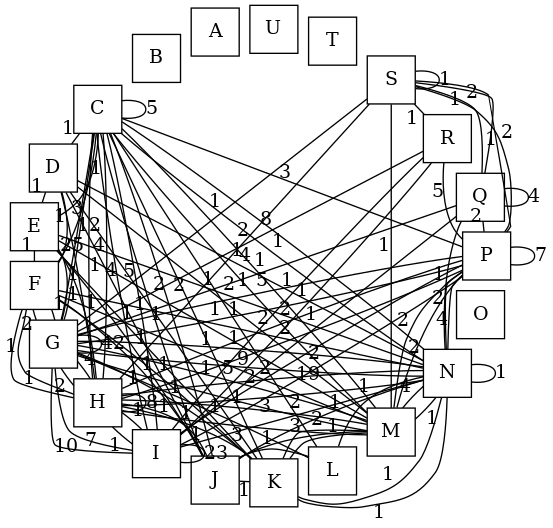
\includegraphics[width=0.33\textwidth]{2021-01.png}} 
%    \subfigure[April 2022]{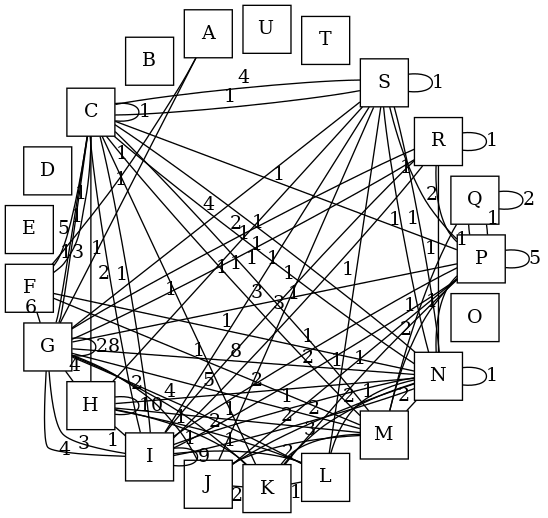
\includegraphics[width=0.33\textwidth]{2022-04.png}} 
%    \subfigure[April 2024]{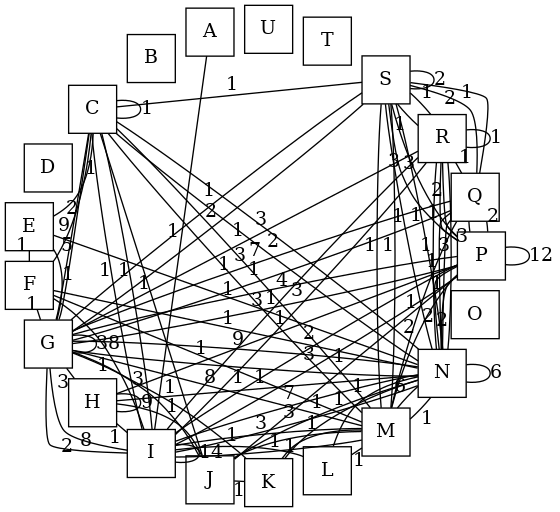
\includegraphics[width=0.33\textwidth]{2024-04.png}}
%    \caption{The temporal dynamic graph of economic activities}
%    \label{fig:foobar}
%\end{figure}
\begin{figure}[h]
    \centering
    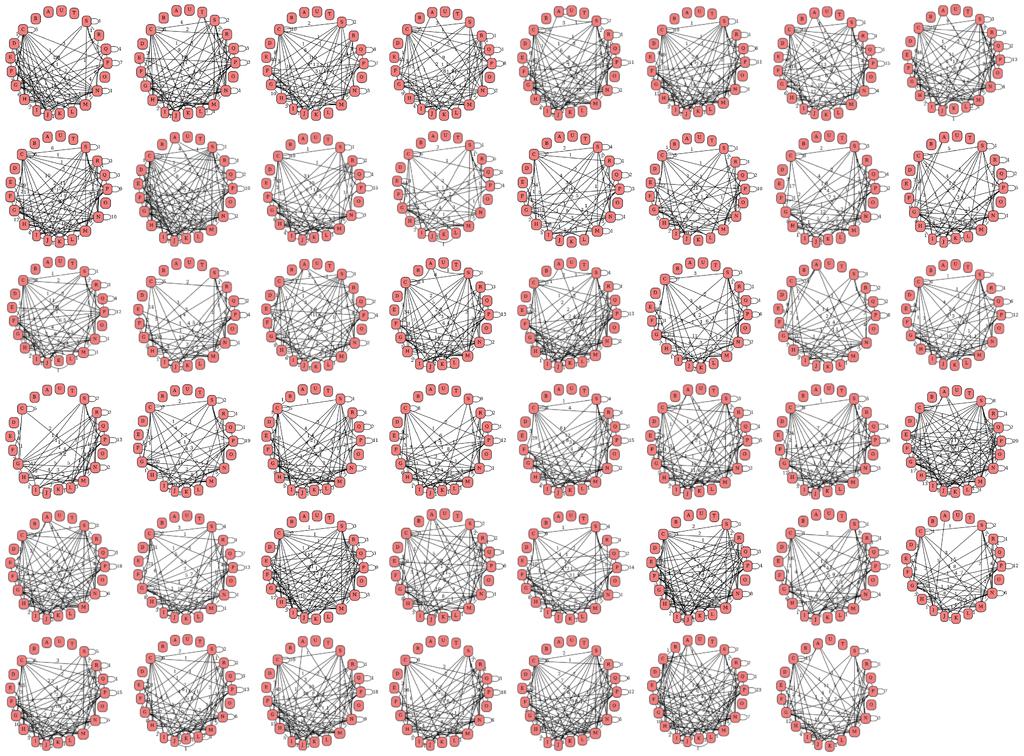
\includegraphics[width=0.75\linewidth]{montage.png}
    \caption{Dynamic Graph}
    \label{fig:dg}
\end{figure}

The edge attributes selected were the number of firms in each AS and the total area consumed by the financial activities in a specific AS. The objective is to analyze the temporal tendency of vertex attributes. This analysis, which depends on the properties of the topological graph, differs from the traditional temporal analysis.

\subsection{Data Pipeline} 
The finding of frequent subgraphs is a complex task, because of its huge search space. The algorithm gSpan \cite{yan2002gspan} eliminates candidate generation and combines the isomorphism test and subgraph growth into one function. This strategy enables good performance. Frequent subgraphs are important to discover how the activities interact to create a firm. The problem in processing the dynamic graph is the edge weight, which represents the intensity of firms in a single period. To tackle this issue the study utilizes a simple fuzzy function to discrete the values. Values less than five are considered Low, values greater than five and lower than fifteen are considered Medium, and higher values are considered High.

The frequent pattern mining algorithm can generate many patterns, depending on its parameter settings. Most candidate patterns often share identical or highly similar topological structures. To address this, our study employs a combination of the Simple Baseline Algorithm for Graph Classification and Graph Embedding (SF) \cite{de2018simple} to construct the embedding space. This method is efficient and computationally simple, leveraging the spectral decomposition of the graph Laplacian and selecting the $k$ lowest eigenvalues. However, the resulting embedding space suffers from the curse of dimensionality \cite{zaki2020data}, where distances between data points tend to become uniformly distributed over a high-dimensional space, particularly resembling a hemisphere.

To mitigate this issue and reduce the dimensionality, we applied UMAP (Uniform Manifold Approximation and Projection) \cite{mcinnes2018umap}, a robust and scalable manifold learning technique. UMAP effectively reduces the high-dimensional embedding space to a two-dimensional representation, while preserving the underlying structure of the data, respecting the original distances between points.

The reduced embedding space is subsequently processed using HDBSCAN (Hierarchical Density-Based Spatial Clustering of Applications with Noise) \cite{campello2013density}, a density-based hierarchical clustering algorithm. HDBSCAN requires only the minimum number of points per cluster as a key parameter, making it straightforward to configure. The resulting clusters represent groups of subgraphs with similar topological structures. Concentrating patterns within clusters and selecting the most representative pattern, enhances knowledge discovery, reduces the overall number of patterns, and highlights the most informative \cite{SciPyProceedings_11} subgraph structures.

\section{Dataset Limitations and Potential Biases}
\section{Results}
\subsection{Dynamic Graph}

The assortativity of a graph measures the tendency of nodes in the graph to connect with other nodes that are similar to them in some way. In the context of firm theory, some activities are necessary for others, which could indicate that some firms are more important. It is commonly used in network analysis to quantify the extent to which similar nodes (by degree, attributes, or other criteria) are connected. Disassortative graphs (negative assortativity) may indicate complementary relationships among economic activities, where diverse sectors depend on each other.
It is defined in terms of the Pearson correlation coefficient $r$ between the degrees of connected nodes weighted by the crisp value of the number of firms.
\begin{figure}[H]
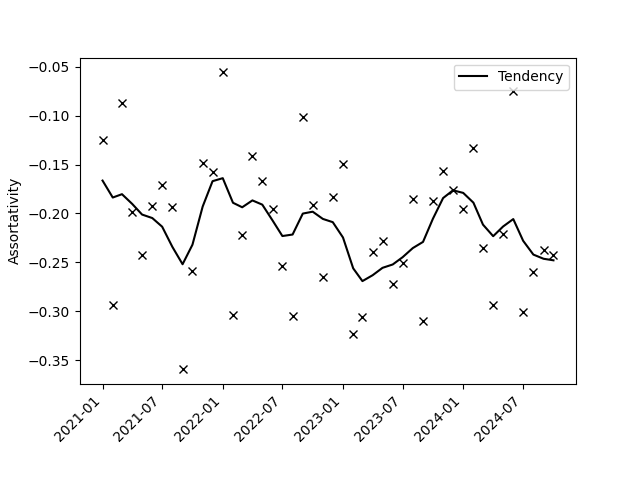
\includegraphics[width=10cm]{assorativity.png}
\centering
 \caption{The assortativity temporal evolution}
    \label{fig:assortativity}
\end{figure}

Figure \ref{fig:assortativity} illustrates the temporal evolution of assortativity, all edges are weighted as one, to analyze only the graph struct. The negative values indicate that all graphs exhibit disassortativity mixing, suggesting that dissimilar nodes are more likely to form connections. This result highlights the significance of economic activities as central hubs influencing others.

The topological time evolution depicted in Figure \ref{fig:tp} was derived by reducing the dimensionality using the UMAP with the Manhattan distance metric of the 128-dimensional embedding space, generated through SF, to a single dimension. All edges are weighted as in the previous example for the same purpose. The results suggest a periodic behavior, indicating that certain frequent subgraphs may hold greater significance than others due to their time-dependent characteristics.

\begin{figure}[H]
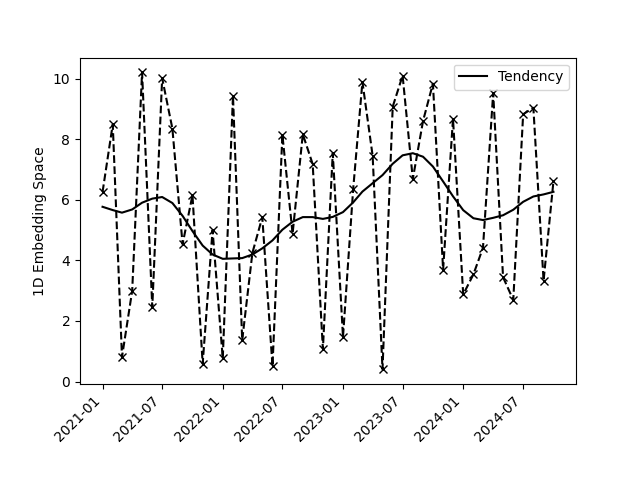
\includegraphics[width=10cm]{time_struct.png}
\centering
 \caption{Topological Time Evolving}
    \label{fig:tp}
\end{figure}

\subsection{Frequent Subgraph Mining}

The gSpan algorithm was configured with a minimum support threshold of $50\%$, as Figure \ref{fig:tp} suggests the presence of two distinct graph clusters and not seeking one edge graph because the study is more interested in relations. This configuration yielded $1,180$ patterns, ranked by FSP-Rank \cite{ur2021graph} with weight 0, because this metric depends only on graph parameters, not necessitating generating random graphs to compare. This result is important to find the Economic Network Motifs. Motifs are recurrent and statistically significant subgraphs of a larger graph. In an economic context, these patterns are the set of firms each commonly share activities over a network, this indicates how the monopoly or oligopoly could naturally emerge from how an activity is shared between firms. All graphs in Figures \ref{grf:freq_r1} and \ref{grf:freq_r2} were the most ranked patterns with a value of 0.5.

\begin{figure}[H]
\centering
\begin{tabular}{ccc}
%%%%%%%%%%%%%%%%%%%%%% 1 %%%%%%%%%%%%%%%%%%%%%%%%%%%%%%%%%%%
\subfigure [Support $100\%$] {
  \resizebox{0.28\textwidth}{!}{%
      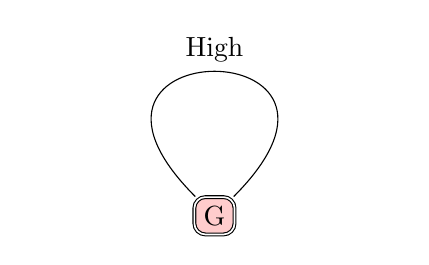
\begin{tikzpicture}[scale=6]
      \draw
        (-1.0, 0.0) node[fill=red!20,draw,double,rounded corners] (0){G};
      \begin{scope}[-]
        \draw[loop, above] (0) to node[] {High} (1);
      \end{scope}
    \end{tikzpicture} 
    }
} &
%%%%%%%%%%%%%%%%%%%%%% 2 %%%%%%%%%%%%%%%%%%%%%%%%%%%%%%%%%%%
\subfigure [Support $87\%$] {
  \resizebox{0.28\textwidth}{!}{%
    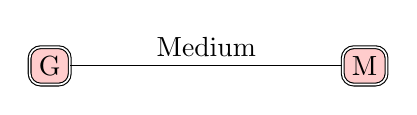
\begin{tikzpicture}[scale=2]
      \draw
        (-1.0, 0.0) node[fill=red!20,draw,double,rounded corners] (0){G}
        (1.0, 0.0) node[fill=red!20,draw,double,rounded corners] (1){M};
      \begin{scope}[-]
        \draw[above] (0) to node[] {Medium} (1);
      \end{scope}
    \end{tikzpicture} 
    }
}

%%%%%%%%%%%%%%%%%%%%%% 4 %%%%%%%%%%%%%%%%%%%%%%%%%%%%%%%%%%%
\subfigure [Support $87\%$] {

  \resizebox{0.28\textwidth}{!}{%
      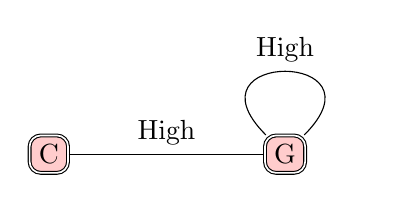
\begin{tikzpicture}[scale=1.5]
       \draw
        (-1.0, 0.0) node[fill=red!20,draw,double,rounded corners] (0){C}
        (1.0, 0.0) node[fill=red!20,draw,double,rounded corners] (1){G};
      \begin{scope}[-]
        \draw[above] (0) to node[] {High} (1);
        \draw[loop,above] (1) to node[] {High} (1);
      \end{scope}
    \end{tikzpicture}

    }
} \\
\end{tabular}
\caption{Most Frequent Patterns}
\label{grf:freq}
\end{figure}

\begin{figure}[H]
\centering
\begin{tabular}{ccc}
%%%%%%%%%%%%%%%%%%%%%% 1 %%%%%%%%%%%%%%%%%%%%%%%%%%%%%%%%%%%
\subfigure [Support $57\%$] {
  \resizebox{0.28\textwidth}{!}{%
      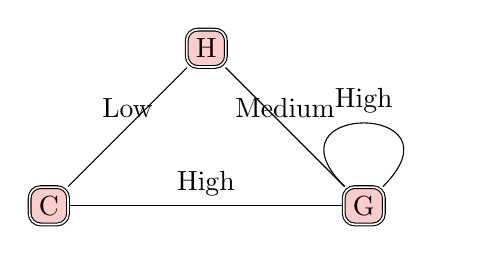
\begin{tikzpicture}[scale=2]
      \draw
        (-1.0, -0.333) node[fill=red!20,draw,double,rounded corners] (0){C}
        (1.0, -0.333) node[fill=red!20,draw,double,rounded corners] (1){G}
        (0.0, 0.667) node[fill=red!20,draw,double,rounded corners] (2){H};
      \begin{scope}[-,above]
        \draw (0) to node[] {High} (1);
        \draw (0) to node[] {Low} (2) ;
        \draw[loop,] (1) to node[] {High} (1);
        \draw (1) to node[] {Medium} (2);
      \end{scope}
     
    \end{tikzpicture} 
    }
} &
%%%%%%%%%%%%%%%%%%%%%% 2 %%%%%%%%%%%%%%%%%%%%%%%%%%%%%%%%%%%
\subfigure [Support $55\%$] {
  \resizebox{0.28\textwidth}{!}{%
    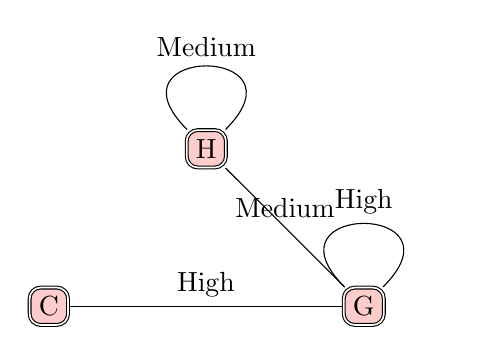
\begin{tikzpicture}[scale=2]
      \draw
        (-1.0, -0.333) node[fill=red!20,draw,double,rounded corners] (0){C}
        (1.0, -0.333) node[fill=red!20,draw,double,rounded corners] (1){G}
        (0.0, 0.667) node[fill=red!20,draw,double,rounded corners] (2){H};
      \begin{scope}[-,above]
        \draw (0) to node[] {High} (1);
        \draw[loop,] (1) to node[] {High} (1);
        \draw (1) to node[] {Medium} (2);
        \draw[loop,] (2) to node[] {Medium} (2);
      \end{scope}
    \end{tikzpicture} 
    }
}

%%%%%%%%%%%%%%%%%%%%%% 3 %%%%%%%%%%%%%%%%%%%%%%%%%%%%%%%%%%%
\subfigure [Support $55\%$] {
  \resizebox{0.28\textwidth}{!}{%
      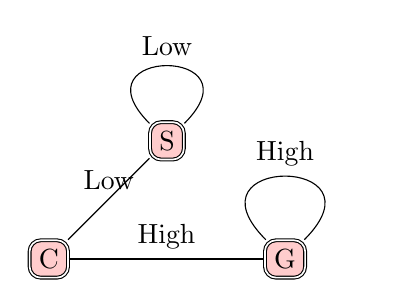
\begin{tikzpicture}[scale=1.5]
      \draw
        (-1.0, -0.333) node[fill=red!20,draw,double,rounded corners] (0){C}
        (1.0, -0.333) node[fill=red!20,draw,double,rounded corners] (1){G}
        (0.0, 0.667) node[fill=red!20,draw,double,rounded corners] (2){S};
      \begin{scope}[-,above]
        \draw (0) to node[] {High} (1);
        \draw (0) to node[] {Low} (2);
        \draw[loop,] (1) to node[] {High} (1);
        \draw[loop,] (2) to node[] {Low} (2);
      \end{scope}
    \end{tikzpicture}

    }
} \\
\end{tabular}
\caption{Part 1: Most FSP Ranked Patterns}
\label{grf:freq_r1}
\end{figure}

\begin{figure}[H]
\centering
\begin{tabular}{ccc}
%%%%%%%%%%%%%%%%%%%%%% 1 %%%%%%%%%%%%%%%%%%%%%%%%%%%%%%%%%%%
\subfigure [Support $55\%$] {
  \resizebox{0.28\textwidth}{!}{%
      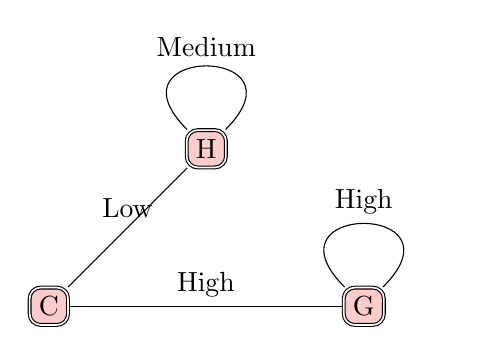
\begin{tikzpicture}[scale=2]
      \draw
        (-1.0, -0.333) node[fill=red!20,draw,double,rounded corners] (0){C}
        (1.0, -0.333) node[fill=red!20,draw,double,rounded corners] (1){G}
        (0.0, 0.667) node[fill=red!20,draw,double,rounded corners] (2){H};
      \begin{scope}[-,above]
        \draw (0) to node[] {High} (1);
        \draw (0) to node[] {Low} (2);
        \draw[loop,] (1) to node[] {High} (1);
        \draw[loop,] (2) to node[] {Medium} (2);
      \end{scope}
     
    \end{tikzpicture} 
    }
} &
%%%%%%%%%%%%%%%%%%%%%% 2 %%%%%%%%%%%%%%%%%%%%%%%%%%%%%%%%%%%
\subfigure [Support $55\%$] {
  \resizebox{0.28\textwidth}{!}{%
    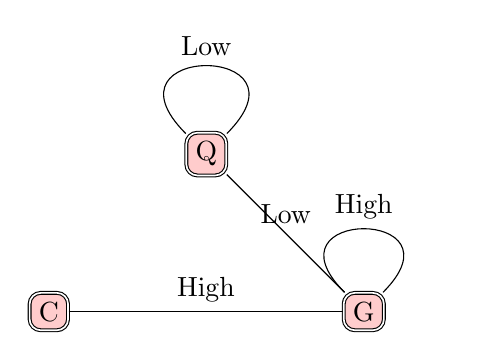
\begin{tikzpicture}[scale=2]
        \draw
        (-1.0, -0.333) node[fill=red!20,draw,double,rounded corners] (0){C}
        (1.0, -0.333) node[fill=red!20,draw,double,rounded corners] (1){G}
        (0.0, 0.667) node[fill=red!20,draw,double,rounded corners] (2){Q};
      \begin{scope}[-,above]
        \draw (0) to node[] {High} (1);
        \draw[loop,] (1) to node[] {High} (1);
        \draw (1) to node[] {Low} (2);
        \draw[loop,] (2) to node[] {Low} (2);
      \end{scope}

    \end{tikzpicture} 
    }
}

%%%%%%%%%%%%%%%%%%%%%% 3 %%%%%%%%%%%%%%%%%%%%%%%%%%%%%%%%%%%
\subfigure [Support $51\%$] {
  \resizebox{0.28\textwidth}{!}{%
      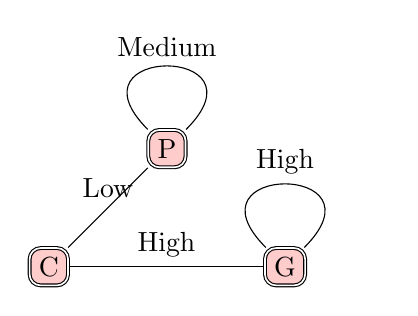
\begin{tikzpicture}[scale=1.5]
      \draw
        (-1.0, -0.333) node[fill=red!20,draw,double,rounded corners] (0){C}
        (1.0, -0.333) node[fill=red!20,draw,double,rounded corners] (1){G}
        (0.0, 0.667) node[fill=red!20,draw,double,rounded corners] (2){P};
      \begin{scope}[-,above]
        \draw (0) to node[] {High} (1);
        \draw (0) to node[] {Low} (2);
        \draw[loop,] (1) to node[] {High} (1);
        \draw[loop,] (2) to node[] {Medium} (2);
      \end{scope}
      
    \end{tikzpicture}

    }
} \\
\end{tabular}
\caption{Part 2: Most FSP Ranked Patterns}
\label{grf:freq_r2}
\end{figure}

The FSP-Rank metric focuses solely on the graph topology to enhance ranking. This study adapted the graph weights W to represent the weighted average of edge crisp values, with weights set to one, five, and fifteen. However, this approach does not account for the support value. A new ranking method, the Euclidean norm of support and weighted rank $|| \mathcal{R} ||_{2}$ was proposed to address this limitation.

\begin{figure}[H]
\centering
\begin{tabular}{ccc}
%%%%%%%%%%%%%%%%%%%%%% 1 %%%%%%%%%%%%%%%%%%%%%%%%%%%%%%%%%%%
\subfigure [ $|| \mathcal{R} ||_{2}$ $2.22$] {
  \resizebox{0.28\textwidth}{!}{%
      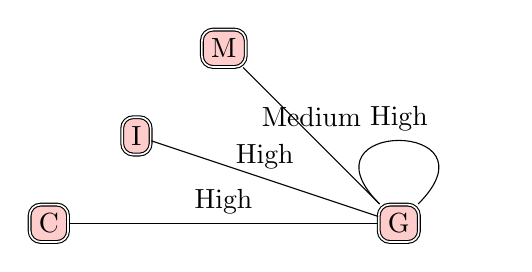
\begin{tikzpicture}[scale=2.5]
      \draw
        (-0.778, -0.333) node[fill=red!20,draw,double,rounded corners] (0){C}
        (1.0, -0.333) node[fill=red!20,draw,double,rounded corners] (1){G}
        (-0.333, 0.111) node[fill=red!20,draw,double,rounded corners] (2){I}
        (0.111, 0.556) node[fill=red!20,draw,double,rounded corners] (3){M};
      \begin{scope}[-,above]
        \draw (0) to node[] {High} (1);
        \draw[loop,] (1) to node[] {High} (1);
        \draw (1) to node[] {High} (2);
        \draw (1) to node[] {Medium} (3);
      \end{scope}
    \end{tikzpicture}
    }
} &
%%%%%%%%%%%%%%%%%%%%%% 2 %%%%%%%%%%%%%%%%%%%%%%%%%%%%%%%%%%%
\subfigure [$|| \mathcal{R} ||_{2}$ $2.14$] {
  \resizebox{0.28\textwidth}{!}{%
    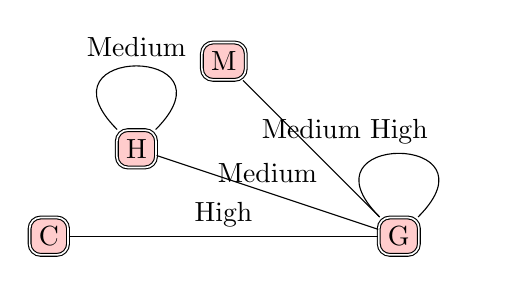
\begin{tikzpicture}[scale=2.5]
      \draw
        (-0.778, -0.333) node[fill=red!20,draw,double,rounded corners] (0){C}
        (1.0, -0.333) node[fill=red!20,draw,double,rounded corners] (1){G}
        (-0.333, 0.111) node[fill=red!20,draw,double,rounded corners] (2){H}
        (0.111, 0.556) node[fill=red!20,draw,double,rounded corners] (3){M};
      \begin{scope}[-,above]
        \draw (0) to node[] {High} (1);
        \draw[loop,] (1) to node[] {High} (1);
        \draw (1) to node[] {Medium} (2);
        \draw (1) to node[] {Medium} (3);
        \draw[loop,] (2) to node[] {Medium} (2);
      \end{scope}
    \end{tikzpicture} 
    }
}

%%%%%%%%%%%%%%%%%%%%%% 3 %%%%%%%%%%%%%%%%%%%%%%%%%%%%%%%%%%%
\subfigure [[$|| \mathcal{R} ||_{2}$ $2.06$] {
  \resizebox{0.28\textwidth}{!}{%
       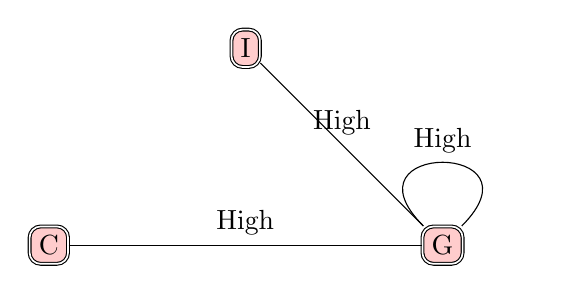
\begin{tikzpicture}[scale=2.5]
      \draw
        (-1.0, -0.333) node[fill=red!20,draw,double,rounded corners] (0){C}
        (1.0, -0.333) node[fill=red!20,draw,double,rounded corners] (1){G}
        (0.0, 0.667) node[fill=red!20,draw,double,rounded corners] (2){I};
      \begin{scope}[-,above]
        \draw (0) to node[] {High} (1);
        \draw[loop,] (1) to node[] {High} (1);
        \draw (1) to node[] {High} (2);
      \end{scope}
    \end{tikzpicture}

    }
} \\
\end{tabular}
\caption{Most Ranked $|| \mathcal{R} ||_{2}$ Patterns}
\label{grf:freq_RR2}
\end{figure}

The results highlight the central role of trading activity in shaping the economic outcomes of Belo Horizonte. As \cite{thia2016trade} asserts, urbanization is a significant driver of international trade, fostering increased intra-industry trade within modern sectors. Furthermore, the study emphasizes the need to address domestic trade costs, as high costs can diminish productivity gains and undermine a country’s capacity to compete in contemporary industries. \cite{faisal2018electricity} affirms there is substantial evidence of co-integration among trade, electricity consumption, economic growth, and urbanization in Iceland. Economic development, trade, and urbanization positively influence short- and long-term electricity consumption. Notably, urbanization emerges as the primary factor driving electricity consumption.

Trading is crucial in manufacturing and professional, scientific, and technical activities. These relationships encompass various services, from bakeries to car workshops. The relationship between trading and manufacturing is significant to other services like education, human health, accommodations, and food services.

To organize these results an exhaustive search was conducted within a constrained parameter space of $1344$ possibles, to determine the optimal configuration. The evaluation metric used was the Hopkins statistic \cite{banerjee2004validating} with a sample size of 58 (about 5\% as recommended in \cite{lawson1990new}). To simplify the process each edge was weighted equally to one.

The optimal configuration achieved a Hopkins score of $0.9976 \pm 0.0002$, indicating near-perfect clustering, as one score corresponds to an ideal clustering dataset. The final configuration was: 10 embedding dimensions for SF, and the UMAP configuration included the following parameters: the number of neighbors set to 200, the minimum distance of 0.5, the number of projected dimensions space equal to 2, and the Euclidean distance metric. It was identified that both algorithms are very susceptible to initial random values, leading to different numbers of clusters, so the initial random seed was set to a fixed value of 10 for UMAP and 48 for SF, for reproducibility.

The clustering configuration process was developed using a randomized search, with configurations ranked by the Silhouette Score. The process achieved an excellent score of $0.945$; as the value one indicates a perfect clustering. The optimal configuration included the following parameters: minimum cluster size and minimum samples of $5$, and cluster selection epsilon of $0.099$.

The high Hopkins Score allows evaluating eccentricity metrics described in Table \ref{tab:clresult} to infer cluster quality, even if HDBSCAN is a pure hierarchical density algorithm.

\begin{figure}[ht]
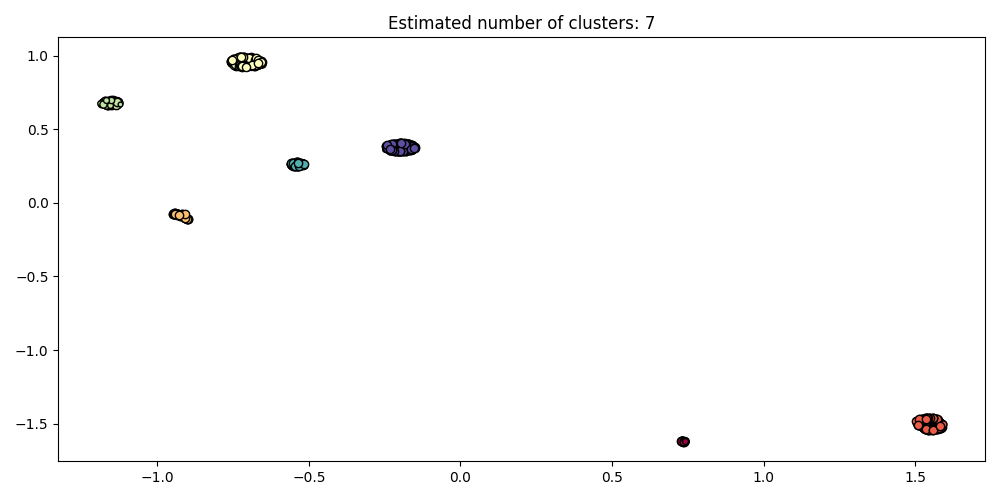
\includegraphics[width=15cm]{cluster.png}
\centering
 \caption{2-D embedding space, each color represents a cluster}
    \label{fig:cluster}
\end{figure}

 

\begin{table}[ht]
\begin{minipage}{\textwidth}
\centering
\vspace{3mm}
\begin{tabular}{cl}
\textbf{Metric} & \textbf{Value} \\
\hline
\textbf{Silhouette} \footnote{Values near 1.0 is better} & $0.939$ \\ 
\textbf{Calinski-Harabasz} \footnote{Higher values is better} & $586,177.94$ \\ 
\textbf{Davies-Bouldin} \footnote{Values near 0.0 is better} & $0.071$ \\ 
\textbf{Clusters} & $7$ \\
\textbf{Outliers} & $0$ \\
\hline
\hline
\end{tabular}
\caption{Cluster quality}
\label{tab:clresult}
\end{minipage}
\end{table}

\begin{table}[H]
\addtolength{\tabcolsep}{-2pt}
\begin{minipage}{\textwidth}
\centering
\vspace{3mm}
\begin{tabular}{ccccccc}
\textbf{Cluster} & \textbf{Assortativity}\footnote{\label{note1}Mean and Standart Desviation} & \textbf{Nodes}\footnoteref{note1} & \textbf{Density}\footnoteref{note1} & \textbf{Diameter}\footnoteref{note1} & \textbf{Max Degree}\footnoteref{note1}  & \textbf{Total}   \\
\hline
$0$ & $-0.78 \pm 0.32$ & $5.0 \pm 0.0$ & $0.45 \pm 0.07$ & $2.18 \pm 0.39$ & $4.41 \pm 0.94$ & $22$ \\
$1$ & $-0.18 \pm 0.33$ & $5.0 \pm 0.0$ & $0.44 \pm 0.05$ & $3.40 \pm 0.49$ & $3.18 \pm 0.96$ & $320$ \\
$2$ & $-0.15 \pm 0.33$ & $6.0 \pm 0.0$ & $0.37 \pm 0.03$ & $3.68 \pm 0.65$ & $3.89 \pm 1.07$ & $38$ \\
$3$ & $-0.26 \pm 0.30$ & $4.0 \pm 0.0$ & $0.56 \pm 0.09$ & $2.92 \pm 0.28$ & $2.55 \pm 0.82$ & $323$ \\
$4$ & $-0.75 \pm 0.43$ & $4.0 \pm 0.0$ & $0.56 \pm 0.09$ & $2.00 \pm 0.00$ & $3.27 \pm 0.76$ & $128$ \\
$5$ & $-0.11 \pm 0.21$ & $2.0 \pm 0.0$ & $1.23 \pm 0.42$ & $1.00 \pm 0.00$ & $1.45 \pm 0.84$ & $88$ \\
$6$ & $-0.73 \pm 0.41$ & $3.0 \pm 0.0$ & $0.76 \pm 0.17$ & $1.97 \pm 0.18$ & $2.34 \pm 0.66$ & $261$ \\
\hline
\hline
\end{tabular}

\caption{Clusters metrics}
\label{tab:clrquality}
\end{minipage}
\end{table}


\begin{figure}[H]
\centering
\begin{tabular}{ccc}
%%%%%%%%%%%%%%%%%%%%%% 1 %%%%%%%%%%%%%%%%%%%%%%%%%%%%%%%%%%%
\subfigure [Support 51\% $|| \mathcal{R} ||_{2}$ $1.91$] {
  \resizebox{0.28\textwidth}{!}{%
       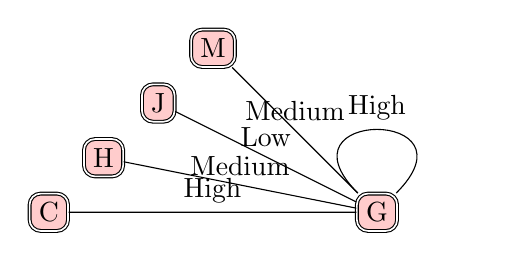
\begin{tikzpicture}[scale=2.5]
      \draw
        (-0.667, -0.333) node[fill=red!20,draw,double,rounded corners] (0){C}
        (1.0, -0.333) node[fill=red!20,draw,double,rounded corners] (1){G}
        (-0.389, -0.056) node[fill=red!20,draw,double,rounded corners] (2){H}
        (-0.111, 0.222) node[fill=red!20,draw,double,rounded corners] (3){J}
        (0.167, 0.5) node[fill=red!20,draw,double,rounded corners] (4){M};
      \begin{scope}[-,above]
        \draw (0) to node[] {High} (1);
        \draw[loop,] (1) to node[] {High} (1);
        \draw (1) to node[] {Medium} (2);
        \draw (1) to node[] {Low} (3);
        \draw (1) to node[] {Medium} (4);
      \end{scope}
    \end{tikzpicture}
    }
} &
%%%%%%%%%%%%%%%%%%%%%% 2 %%%%%%%%%%%%%%%%%%%%%%%%%%%%%%%%%%%
\subfigure [Support 55\% $|| \mathcal{R} ||_{2}$ $1.92$] {
  \resizebox{0.28\textwidth}{!}{%
    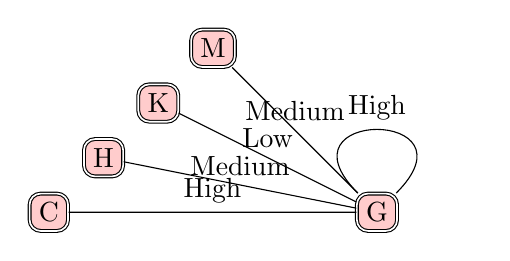
\begin{tikzpicture}[scale=2.5]
      \draw
        (-0.667, -0.333) node[fill=red!20,draw,double,rounded corners] (0){C}
        (1.0, -0.333) node[fill=red!20,draw,double,rounded corners] (1){G}
        (-0.389, -0.056) node[fill=red!20,draw,double,rounded corners] (2){H}
        (-0.111, 0.222) node[fill=red!20,draw,double,rounded corners] (3){K}
        (0.167, 0.5) node[fill=red!20,draw,double,rounded corners] (4){M};
      \begin{scope}[-,above]
        \draw (0) to node[] {High} (1);
        \draw[loop,] (1) to node[] {High} (1);
        \draw (1) to node[] {Medium} (2);
        \draw (1) to node[] {Low} (3);
        \draw (1) to node[] {Medium} (4);
      \end{scope}
    \end{tikzpicture}
    }
} &

%%%%%%%%%%%%%%%%%%%%%% 3 %%%%%%%%%%%%%%%%%%%%%%%%%%%%%%%%%%%
\subfigure [Support 60\%[$|| \mathcal{R} ||_{2}$ $1.93$] {
  \resizebox{0.28\textwidth}{!}{%
       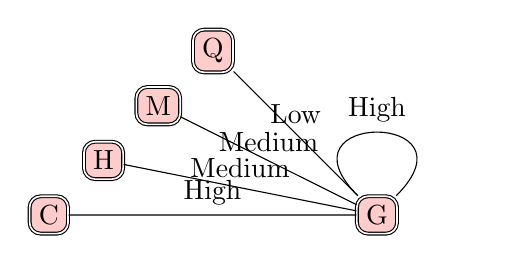
\begin{tikzpicture}[scale=2.5]
      \draw
        (-0.667, -0.333) node[fill=red!20,draw,double,rounded corners] (0){C}
        (1.0, -0.333) node[fill=red!20,draw,double,rounded corners] (1){G}
        (-0.389, -0.056) node[fill=red!20,draw,double,rounded corners] (2){H}
        (-0.111, 0.222) node[fill=red!20,draw,double,rounded corners] (3){M}
        (0.167, 0.5) node[fill=red!20,draw,double,rounded corners] (4){Q};
      \begin{scope}[-,above]
        \draw (0) to node[] {High} (1);
        \draw[loop,] (1) to node[] {High} (1);
        \draw (1) to node[] {Medium} (2);
        \draw (1) to node[] {Medium} (3);
        \draw (1) to node[] {Low} (4);
      \end{scope}
    \end{tikzpicture}

    }
} \\

\end{tabular}
\caption{Cluster 0 Most Ranked $|| \mathcal{R} ||_{2}$ Patterns}
\label{grf:freq_cls0}
\end{figure}


\begin{figure}[H]
\centering
\begin{tabular}{ccc}
%%%%%%%%%%%%%%%%%%%%%% 1 %%%%%%%%%%%%%%%%%%%%%%%%%%%%%%%%%%%
\subfigure [Support 60\% $|| \mathcal{R} ||_{2}$ $1.93$] {
  \resizebox{0.28\textwidth}{!}{%
   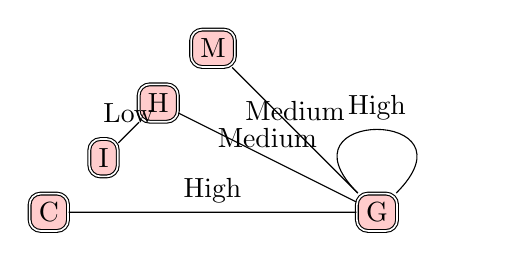
\begin{tikzpicture}[scale=2.5]
      \draw
        (-0.667, -0.333) node[fill=red!20,draw,double,rounded corners] (0){C}
        (1.0, -0.333) node[fill=red!20,draw,double,rounded corners] (1){G}
        (-0.111, 0.222) node[fill=red!20,draw,double,rounded corners] (2){H}
        (-0.389, -0.056) node[fill=red!20,draw,double,rounded corners] (3){I}
        (0.167, 0.5) node[fill=red!20,draw,double,rounded corners] (4){M};
      \begin{scope}[-,above]
        \draw (0) to node[] {High} (1);
        \draw[loop,] (1) to node[] {High} (1);
        \draw (1) to node[] {Medium} (2);
        \draw (1) to node[] {Medium} (4);
        \draw (2) to node[] {Low} (3);
      \end{scope}
    \end{tikzpicture}

    }
} &
%%%%%%%%%%%%%%%%%%%%%% 2 %%%%%%%%%%%%%%%%%%%%%%%%%%%%%%%%%%%
\subfigure [Support 51\% $|| \mathcal{R} ||_{2}$ $2.05$] {
  \resizebox{0.28\textwidth}{!}{%
     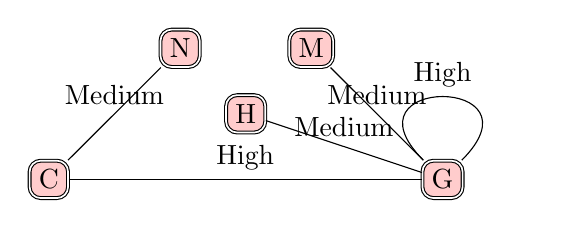
\begin{tikzpicture}[scale=2.5]
      \draw
        (-1.0, -0.333) node[fill=red!20,draw,double,rounded corners] (0){C}
        (1.0, -0.333) node[fill=red!20,draw,double,rounded corners] (1){G}
        (0.0, 0.0) node[fill=red!20,draw,double,rounded corners] (2){H}
        (0.333, 0.333) node[fill=red!20,draw,double,rounded corners] (3){M}
        (-0.333, 0.333) node[fill=red!20,draw,double,rounded corners] (4){N};
      \begin{scope}[-,above]
        \draw (0) to node[] {High} (1);
        \draw (0) to node[] {Medium} (4);
        \draw[loop,] (1) to node[] {High} (1);
        \draw (1) to node[] {Medium} (2);
        \draw (1) to node[] {Medium} (3);
      \end{scope}
    \end{tikzpicture}
    }
} &

%%%%%%%%%%%%%%%%%%%%%% 3 %%%%%%%%%%%%%%%%%%%%%%%%%%%%%%%%%%%
\subfigure [Support 53\% $|| \mathcal{R} ||_{2}$ $2.05$] {
  \resizebox{0.28\textwidth}{!}{%
           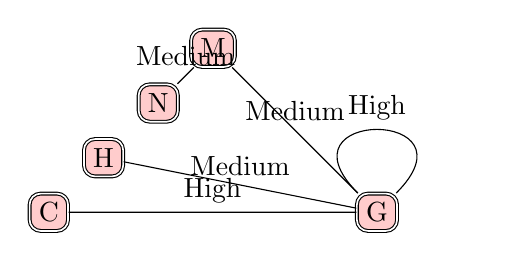
\begin{tikzpicture}[scale=2.5]
      \draw
        (-0.667, -0.333) node[fill=red!20,draw,double,rounded corners] (0){C}
        (1.0, -0.333) node[fill=red!20,draw,double,rounded corners] (1){G}
        (-0.389, -0.056) node[fill=red!20,draw,double,rounded corners] (2){H}
        (0.167, 0.5) node[fill=red!20,draw,double,rounded corners] (3){M}
        (-0.111, 0.222) node[fill=red!20,draw,double,rounded corners] (4){N};
      \begin{scope}[-,above]
        \draw (0) to node[] {High} (1);
        \draw[loop,] (1) to node[] {High} (1);
        \draw (1) to node[] {Medium} (2);
        \draw (1) to node[] {Medium} (3);
        \draw (3) to node[] {Medium} (4);
      \end{scope}
    \end{tikzpicture}

    }
} \\

\end{tabular}
\caption{Cluster 1 Most Ranked $|| \mathcal{R} ||_{2}$ Patterns}
\label{grf:freq_cls1}
\end{figure}

\begin{figure}[H]
\centering
\begin{tabular}{ccc}
%%%%%%%%%%%%%%%%%%%%%% 1 %%%%%%%%%%%%%%%%%%%%%%%%%%%%%%%%%%%
\subfigure [Support 51\% $|| \mathcal{R} ||_{2}$ $1.94$] {
  \resizebox{0.28\textwidth}{!}{%
  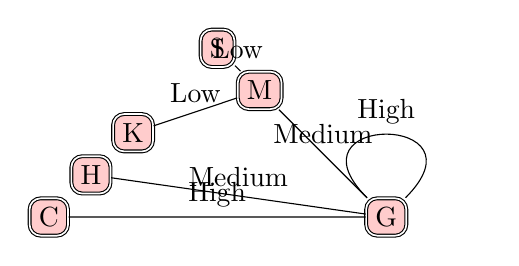
\begin{tikzpicture}[scale=2.5]
      \draw
        (-0.714, -0.357) node[fill=red!20,draw,double,rounded corners] (0){C}
        (1.0, -0.357) node[fill=red!20,draw,double,rounded corners] (1){G}
        (-0.5, -0.143) node[fill=red!20,draw,double,rounded corners] (2){H}
        (0.357, 0.286) node[fill=red!20,draw,double,rounded corners] (3){M}
        (-0.286, 0.071) node[fill=red!20,draw,double,rounded corners] (4){K}
        (0.143, 0.5) node[fill=red!20,draw,double,rounded corners] (5){S};
      \begin{scope}[-,above]
        \draw (0) to node[] {High} (1);
        \draw[loop,] (1) to node[] {High} (1);
        \draw (1) to node[] {Medium} (2);
        \draw (1) to node[] {Medium} (3);
        \draw (3) to node[] {Low} (4);
        \draw (3) to node[] {Low} (5);
      \end{scope}
    \end{tikzpicture}

    }
} &
%%%%%%%%%%%%%%%%%%%%%% 2 %%%%%%%%%%%%%%%%%%%%%%%%%%%%%%%%%%%
\subfigure [Support 51\% $|| \mathcal{R} ||_{2}$ $1.94$] {
  \resizebox{0.28\textwidth}{!}{%
     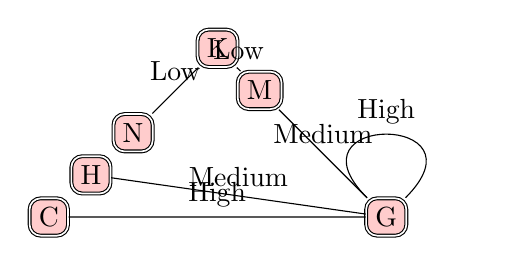
\begin{tikzpicture}[scale=2.5]
      \draw
        (-0.714, -0.357) node[fill=red!20,draw,double,rounded corners] (0){C}
        (1.0, -0.357) node[fill=red!20,draw,double,rounded corners] (1){G}
        (-0.5, -0.143) node[fill=red!20,draw,double,rounded corners] (2){H}
        (0.357, 0.286) node[fill=red!20,draw,double,rounded corners] (3){M}
        (0.143, 0.5) node[fill=red!20,draw,double,rounded corners] (4){K}
        (-0.286, 0.071) node[fill=red!20,draw,double,rounded corners] (5){N};
      \begin{scope}[-,above]
        \draw (0) to node[] {High} (1);
        \draw[loop,] (1) to node[] {High} (1);
        \draw (1) to node[] {Medium} (2);
        \draw (1) to node[] {Medium} (3);
        \draw (3) to node[] {Low} (4);
        \draw (4) to node[] {Low} (5);
      \end{scope}
    \end{tikzpicture}

    }
} &

%%%%%%%%%%%%%%%%%%%%%% 3 %%%%%%%%%%%%%%%%%%%%%%%%%%%%%%%%%%%
\subfigure [Support 53\% $|| \mathcal{R} ||_{2}$ $1.95$] {
  \resizebox{0.28\textwidth}{!}{%
           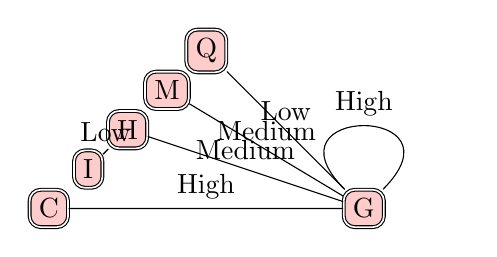
\begin{tikzpicture}[scale=2.5]
      \draw
        (-0.6, -0.333) node[fill=red!20,draw,double,rounded corners] (0){C}
        (1.0, -0.333) node[fill=red!20,draw,double,rounded corners] (1){G}
        (-0.2, 0.067) node[fill=red!20,draw,double,rounded corners] (2){H}
        (-0.4, -0.133) node[fill=red!20,draw,double,rounded corners] (3){I}
        (0.0, 0.267) node[fill=red!20,draw,double,rounded corners] (4){M}
        (0.2, 0.467) node[fill=red!20,draw,double,rounded corners] (5){Q};
      \begin{scope}[-,above]
        \draw (0) to node[] {High} (1);
        \draw[loop,] (1) to node[] {High} (1);
        \draw (1) to node[] {Medium} (2);
        \draw (1) to node[] {Medium} (4);
        \draw (1) to node[] {Low} (5);
        \draw (2) to node[] {Low} (3);
      \end{scope}
    \end{tikzpicture}
    }
} \\

\end{tabular}
\caption{Cluster 2 Most Ranked $|| \mathcal{R} ||_{2}$ Patterns}
\label{grf:freq_cls2}
\end{figure}

\begin{figure}[H]
\centering
\begin{tabular}{ccc}
%%%%%%%%%%%%%%%%%%%%%% 1 %%%%%%%%%%%%%%%%%%%%%%%%%%%%%%%%%%%
\subfigure [Support 51\% $|| \mathcal{R} ||_{2}$ $2.00$] {
  \resizebox{0.28\textwidth}{!}{%
  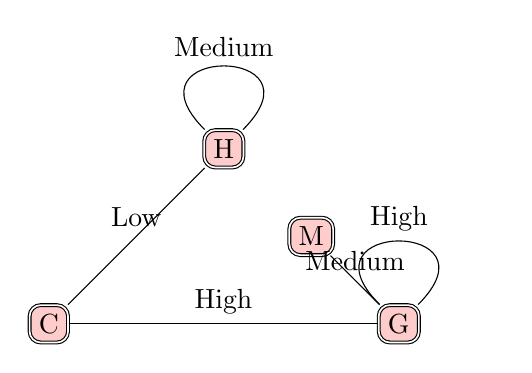
\begin{tikzpicture}[scale=2.5]
      \draw
        (-1.0, -0.333) node[fill=red!20,draw,double,rounded corners] (0){C}
        (0.778, -0.333) node[fill=red!20,draw,double,rounded corners] (1){G}
        (0.333, 0.111) node[fill=red!20,draw,double,rounded corners] (2){M}
        (-0.111, 0.556) node[fill=red!20,draw,double,rounded corners] (3){H};
      \begin{scope}[-,above]
        \draw (0) to node[] {High} (1);
        \draw (0) to node[] {Low} (3);
        \draw[loop,] (1) to node[] {High} (1);
        \draw (1) to node[] {Medium} (2);
        \draw[loop,] (3) to node[] {Medium} (3);
      \end{scope}
    \end{tikzpicture}

    }
} &
%%%%%%%%%%%%%%%%%%%%%% 2 %%%%%%%%%%%%%%%%%%%%%%%%%%%%%%%%%%%
\subfigure [Support 53\% $|| \mathcal{R} ||_{2}$ $2.00$] {
  \resizebox{0.28\textwidth}{!}{%
    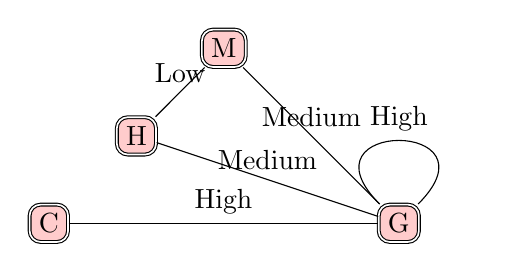
\begin{tikzpicture}[scale=2.5]
      \draw
        (-0.778, -0.333) node[fill=red!20,draw,double,rounded corners] (0){C}
        (1.0, -0.333) node[fill=red!20,draw,double,rounded corners] (1){G}
        (-0.333, 0.111) node[fill=red!20,draw,double,rounded corners] (2){H}
        (0.111, 0.556) node[fill=red!20,draw,double,rounded corners] (3){M};
      \begin{scope}[-,above]
        \draw (0) to node[] {High} (1);
        \draw[loop,] (1) to node[] {High} (1);
        \draw (1) to node[] {Medium} (2);
        \draw (1) to node[] {Medium} (3);
        \draw (2) to node[] {Low} (3);
      \end{scope}
    \end{tikzpicture}

    }
} &

%%%%%%%%%%%%%%%%%%%%%% 3 %%%%%%%%%%%%%%%%%%%%%%%%%%%%%%%%%%%
\subfigure [Support 55\% $|| \mathcal{R} ||_{2}$ $2.01$] {
  \resizebox{0.28\textwidth}{!}{%
           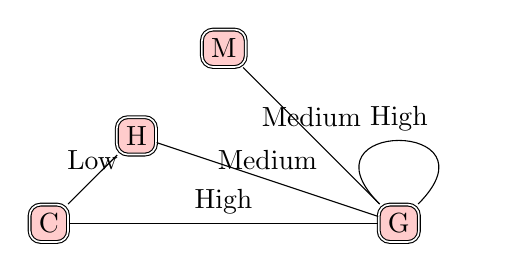
\begin{tikzpicture}[scale=2.5]
      \draw
        (-0.778, -0.333) node[fill=red!20,draw,double,rounded corners] (0){C}
        (1.0, -0.333) node[fill=red!20,draw,double,rounded corners] (1){G}
        (-0.333, 0.111) node[fill=red!20,draw,double,rounded corners] (2){H}
        (0.111, 0.556) node[fill=red!20,draw,double,rounded corners] (3){M};
      \begin{scope}[-,above]
        \draw (0) to node[] {High} (1);
        \draw (0) to node[] {Low} (2);
        \draw[loop,] (1) to node[] {High} (1);
        \draw (1) to node[] {Medium} (2);
        \draw (1) to node[] {Medium} (3);
      \end{scope}
    \end{tikzpicture}
    }
} \\

\end{tabular}
\caption{Cluster 3 Most Ranked $|| \mathcal{R} ||_{2}$ Patterns}
\label{grf:freq_cls3}
\end{figure}

\begin{figure}[h]
\centering
\begin{tabular}{ccc}
%%%%%%%%%%%%%%%%%%%%%% 1 %%%%%%%%%%%%%%%%%%%%%%%%%%%%%%%%%%%
\subfigure [Support 68\% $|| \mathcal{R} ||_{2}$ $1.93$] {
  \resizebox{0.28\textwidth}{!}{%
  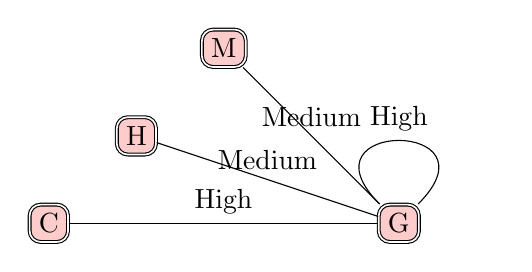
\begin{tikzpicture}[scale=2.5]
      \draw
        (-0.778, -0.333) node[fill=red!20,draw,double,rounded corners] (0){C}
        (1.0, -0.333) node[fill=red!20,draw,double,rounded corners] (1){G}
        (-0.333, 0.111) node[fill=red!20,draw,double,rounded corners] (2){H}
        (0.111, 0.556) node[fill=red!20,draw,double,rounded corners] (3){M};
      \begin{scope}[-,above]
        \draw (0) to node[] {High} (1);
        \draw[loop,] (1) to node[] {High} (1);
        \draw (1) to node[] {Medium} (2);
        \draw (1) to node[] {Medium} (3);
      \end{scope}
    \end{tikzpicture}

    }
} &
%%%%%%%%%%%%%%%%%%%%%% 2 %%%%%%%%%%%%%%%%%%%%%%%%%%%%%%%%%%%
\subfigure [Support 51\% $|| \mathcal{R} ||_{2}$ $2.14$] {
  \resizebox{0.28\textwidth}{!}{%
   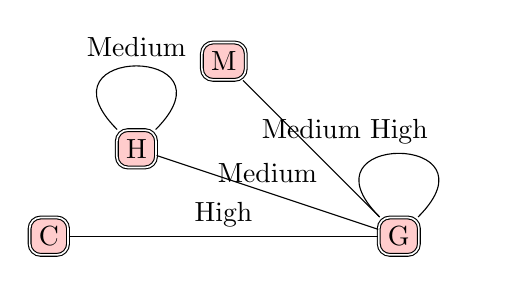
\begin{tikzpicture}[scale=2.5]
      \draw
        (-0.778, -0.333) node[fill=red!20,draw,double,rounded corners] (0){C}
        (1.0, -0.333) node[fill=red!20,draw,double,rounded corners] (1){G}
        (-0.333, 0.111) node[fill=red!20,draw,double,rounded corners] (2){H}
        (0.111, 0.556) node[fill=red!20,draw,double,rounded corners] (3){M};
      \begin{scope}[-,above]
        \draw (0) to node[] {High} (1);
        \draw[loop,] (1) to node[] {High} (1);
        \draw (1) to node[] {Medium} (2);
        \draw (1) to node[] {Medium} (3);
        \draw[loop,] (2) to node[] {Medium} (2);
      \end{scope}
    \end{tikzpicture}

    }
} &

%%%%%%%%%%%%%%%%%%%%%% 3 %%%%%%%%%%%%%%%%%%%%%%%%%%%%%%%%%%%
\subfigure [Support 53\% $|| \mathcal{R} ||_{2}$ $2.20$] {
  \resizebox{0.28\textwidth}{!}{%
          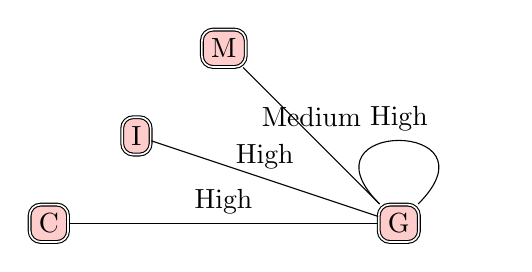
\begin{tikzpicture}[scale=2.5]
      \draw
        (-0.778, -0.333) node[fill=red!20,draw,double,rounded corners] (0){C}
        (1.0, -0.333) node[fill=red!20,draw,double,rounded corners] (1){G}
        (-0.333, 0.111) node[fill=red!20,draw,double,rounded corners] (2){I}
        (0.111, 0.556) node[fill=red!20,draw,double,rounded corners] (3){M};
      \begin{scope}[-,above]
        \draw (0) to node[] {High} (1);
        \draw[loop,] (1) to node[] {High} (1);
        \draw (1) to node[] {High} (2);
        \draw (1) to node[] {Medium} (3);
      \end{scope}
    \end{tikzpicture}

    }
} \\

\end{tabular}
\caption{Cluster 4 Most Ranked $|| \mathcal{R} ||_{2}$ Patterns}
\label{grf:freq_cls4}
\end{figure}

\begin{figure}[h]
\centering
\begin{tabular}{ccc}
%%%%%%%%%%%%%%%%%%%%%% 1 %%%%%%%%%%%%%%%%%%%%%%%%%%%%%%%%%%%
\subfigure [Support 68\% $|| \mathcal{R} ||_{2}$ $1.17$] {
  \resizebox{0.28\textwidth}{!}{%
  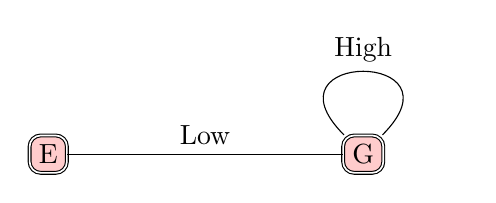
\begin{tikzpicture}[scale=2]
      \draw
        (-1.0, 0.0) node[fill=red!20,draw,double,rounded corners] (0){E}
        (1.0, 0.0) node[fill=red!20,draw,double,rounded corners] (1){G};
      \begin{scope}[-,above]
        \draw (0) to node[] {Low} (1);
        \draw[loop,] (1) to node[] {High} (1);
      \end{scope}
    \end{tikzpicture}

    }
} &
%%%%%%%%%%%%%%%%%%%%%% 2 %%%%%%%%%%%%%%%%%%%%%%%%%%%%%%%%%%%
\subfigure [Support 100\% $|| \mathcal{R} ||_{2}$ $1.23$] {
  \resizebox{0.28\textwidth}{!}{%
    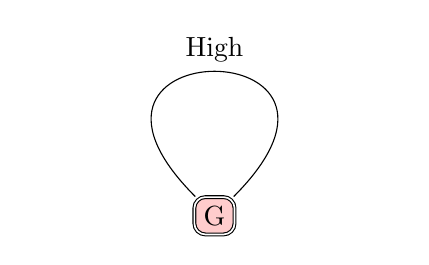
\begin{tikzpicture}[scale=6]
      \draw
        (-1.0, 0.0) node[fill=red!20,draw,double,rounded corners] (0){G};
      \begin{scope}[-]
        \draw[loop, above] (0) to node[] {High} (1);
      \end{scope}
    \end{tikzpicture} 

    }
} &

%%%%%%%%%%%%%%%%%%%%%% 3 %%%%%%%%%%%%%%%%%%%%%%%%%%%%%%%%%%%
\subfigure [Support 87\% $|| \mathcal{R} ||_{2}$ $1.69$] {
  \resizebox{0.28\textwidth}{!}{%
          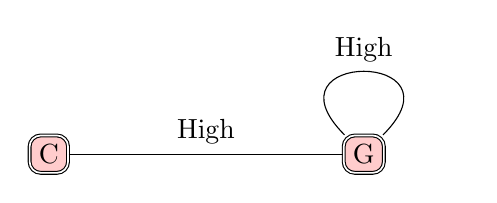
\begin{tikzpicture}[scale=2]
      \draw
        (-1.0, 0.0) node[fill=red!20,draw,double,rounded corners] (0){C}
        (1.0, 0.0) node[fill=red!20,draw,double,rounded corners] (1){G};
      \begin{scope}[-,above]
        \draw (0) to node[] {High} (1);
        \draw[loop,] (1) to node[] {High} (1);
      \end{scope}
    \end{tikzpicture}

    }
} \\

\end{tabular}
\caption{Cluster 5 Most Ranked $|| \mathcal{R} ||_{2}$ Patterns}
\label{grf:freq_cls5}
\end{figure}

\begin{figure}[H]
\centering
\begin{tabular}{ccc}
%%%%%%%%%%%%%%%%%%%%%% 1 %%%%%%%%%%%%%%%%%%%%%%%%%%%%%%%%%%%
\subfigure [Support 57\% $|| \mathcal{R} ||_{2}$ $1.88$] {
  \resizebox{0.28\textwidth}{!}{%
  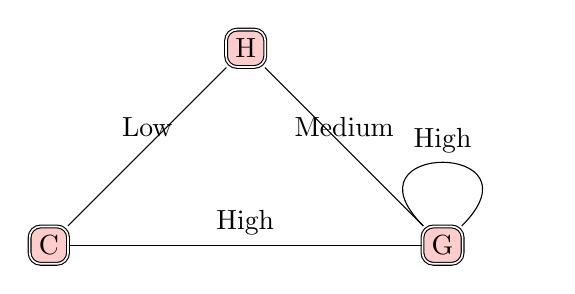
\begin{tikzpicture}[scale=2.5]
      \draw
        (-1.0, -0.333) node[fill=red!20,draw,double,rounded corners] (0){C}
        (1.0, -0.333) node[fill=red!20,draw,double,rounded corners] (1){G}
        (0.0, 0.667) node[fill=red!20,draw,double,rounded corners] (2){H};
      \begin{scope}[-,above]
        \draw (0) to node[] {High} (1);
        \draw (0) to node[] {Low} (2);
        \draw[loop,] (1) to node[] {High} (1);
        \draw (1) to node[] {Medium} (2);
      \end{scope}
    \end{tikzpicture}

    }
} &
%%%%%%%%%%%%%%%%%%%%%% 2 %%%%%%%%%%%%%%%%%%%%%%%%%%%%%%%%%%%
\subfigure [Support 55\% $|| \mathcal{R} ||_{2}$ $2.01$] {
  \resizebox{0.28\textwidth}{!}{%
   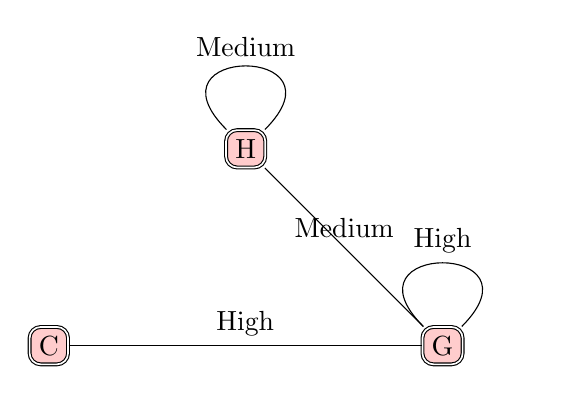
\begin{tikzpicture}[scale=2.5]
      \draw
        (-1.0, -0.333) node[fill=red!20,draw,double,rounded corners] (0){C}
        (1.0, -0.333) node[fill=red!20,draw,double,rounded corners] (1){G}
        (0.0, 0.667) node[fill=red!20,draw,double,rounded corners] (2){H};
      \begin{scope}[-,above]
        \draw (0) to node[] {High} (1);
        \draw[loop,] (1) to node[] {High} (1);
        \draw (1) to node[] {Medium} (2);
        \draw[loop,] (2) to node[] {Medium} (2);
      \end{scope}
    \end{tikzpicture}

    }
} &

%%%%%%%%%%%%%%%%%%%%%% 3 %%%%%%%%%%%%%%%%%%%%%%%%%%%%%%%%%%%
\subfigure [Support 55\% $|| \mathcal{R} ||_{2}$ $2.06$] {
  \resizebox{0.28\textwidth}{!}{%
         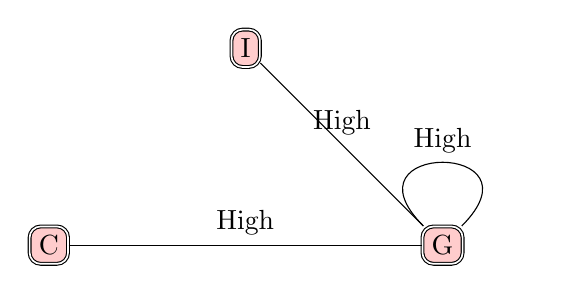
\begin{tikzpicture}[scale=2.5]
      \draw
        (-1.0, -0.333) node[fill=red!20,draw,double,rounded corners] (0){C}
        (1.0, -0.333) node[fill=red!20,draw,double,rounded corners] (1){G}
        (0.0, 0.667) node[fill=red!20,draw,double,rounded corners] (2){I};
      \begin{scope}[-,above]
        \draw (0) to node[] {High} (1);
        \draw[loop,] (1) to node[] {High} (1);
        \draw (1) to node[] {High} (2);
      \end{scope}
    \end{tikzpicture}

    }
} \\

\end{tabular}
\caption{Cluster 6 Most Ranked $|| \mathcal{R} ||_{2}$ Patterns}
\label{grf:freq_cls6}
\end{figure}

The motifs founded was $S_{5}$, $S_{4}$, $S_{3}$, $K_{3}$, and $K_{2}$. The complete graphs of the type $K_{3}$ are: 
\begin{itemize}
  \item Manufacturing (C), trading (G), and transportation (H).
  \item Professional activities (M), trading (G), and transportation (H).
  \item Professional activities (M), administrative and support services (N), and financial, insurance, and related activities (K).
  \item Trading (G), professional activities (M), and information and communication (J).
  \item Trading (G), financial, insurance, and related activities (K), and professional activities (M)
  \item Professional activities (M), administrative and support services (N), and information and communication (J).
\end{itemize}

The star graph pattern $S_{n}$ is the most common graph in clusters zero ($S_{5}$), four ($S_{4}$), and six ($S_{3}$) due to its diameter near two and high disassortativity. These clusters demonstrate how central activities relate to others, one and two present graphs with two connected central vertexes, and finally cluster six shows the higher frequency sub-graph, varying one or two vertexes.

\begin{table}[H]
\addtolength{\tabcolsep}{-2pt}
\centering
\vspace{3mm}
\begin{tabular}{cccc}
\textbf{Cluster} & \textbf{Pattern} & \multicolumn{2}{c}{\textbf{Activity}}\\
\cmidrule(l{.5\tabcolsep}r{.5\tabcolsep}){3-4}
& & \textbf{Central} & \textbf{Peripheral} \\
\hline
\vcenterhead{$0$}{2} & \vcenterhead{$S_{5}$}{2} & M & C, G, H, I, J, K, N, S \\
 &  & G & C, H, J, K, M, Q, S\\
\hline
\vcenterhead{$4$}{9} & \vcenterhead{$S_{4}$}{9} & M & F, G, H, I, J, K, N, P, Q, S\\
&  & G & C, E, H, I, J, K, L, M, P, Q, S\\
&  & J & G, K, M, N, P\\
&  & N & C, F, J, K, M, Q, S \\
&  & H & C, G, I, M, N \\
&  & K & G, H, M, N \\
&  & F & K, M, N \\
&  & S & C, M, N \\
&  & C & G, H, M, N, P, S\\
\hline

\vcenterhead{$6$}{12} & \vcenterhead{$S_{3}$}{12} & N & C, F, H, I, J, K, L, M, P, Q, R, S\\
&  & M & F, G, H, I, J, K, N, P, Q, R, S\\
&  & S & C, F, G, H, I, J, K, M, N, Q\\
&  & I & H, M, N\\
&  & G & C, E, F, H, I, J, K, L, M, N, P, Q, R, S\\
&  & J & C, G, M, N, P\\
&  & C & F, G, H, I, J, N, P, S\\
&  & Q & C, G, H, M, N, P, S\\
&  & P & C, G, J, K, M, Q, R\\
&  & R & G, P\\
&  & F & C, G, H, M, N\\
&  & K & G, H, M, N, P\\
&  & H & C, F, G, I, K, M, N, Q, S\\
\hline
\hline
\end{tabular}
\caption{Description of common stars patterns}
\label{tab:patter046}
\end{table}



\subsection{Dynamic Graph Attributes}

%\subsection{Evaluating}
%\subsection{Deployment}
\section{Conclusion}


The economic urban context of Belo Horizonte is strongly based on trading to supply the demand for products with services or local production. Firms generally are formed by one principal activity with or without a secondary activity. The most shared activities are trading (G), and professional, scientific, and technical activities (M). Policymakers must focus on their needs, such as specialized labor and logistics infrastructure. Graphs (a, and b) in Figure \ref{grf:freq_r1} are important because they represent the supply chain production, trade, and transportation. The intensity of their vertex represents how these services are in high demand in this urban context. Health and education are related demonstrating the importance of providing a good supply chain economic environment. 
\bibliographystyle{sbc}
\bibliography{sbc-template}

\end{document}